\section{Цель работы}
\begin{itemize}
    \item Получить зависимость электрического сопротивления металлического и полупроводникового образцов в диапазоне температур от комнатной до $75^\circ$C.
    \item Вычислить температурный коэффициент сопротивления металла и ширину запрещенной зоны полупроводника.
\end{itemize}

\section{Объект исследования}
\noindent Металлический и полупроводниковый образцы, зависимости их сопротивления от температуры

\section{Метод экспериментального исследования}
\noindent Многократные прямые измерения напряжения на образце и тока, проходящего через него, при различных температурах

\section{Рабочие формулы и исходные данные}
\begin{itemize}
    \item Закон Ома для участка цепи:
    \begin{equation}
        R=\frac{U}{I}
        \label{eqn:OMM}
    \end{equation}
    где R - сопротивление, U - напряжение, I -  сила ток
    \item Cопротивление полупроводника:
    $$R_{\text{п}} = R_m\exp{(\frac{E_g}{2kT})}$$
     где $kT$ - средняя энергия теплового движения, $R_m$ - предел к которому стремится значение сопротивления полупроводника при повышении температуры\\
     
    Прологарифмируем это соотношение и получим формулу для расчета ширины запрещенной зоны (k - постоянная Больцмана, $k=1,38*10^{-23} \textit{ Дж/К}=8,62*10^{-5}\textit{ эВ/К}$):
    \begin{equation}
        E_g=2k \cdot \frac{\Delta \ln({R_{\text{п}}})}{\Delta (1/T)}
    \end{equation}
    \item Зависимость сопротивления от температуры для металла при небольших диапазонах температур:
    \begin{equation}
        R_{\text{м}} = R_0(1+\alpha T),
    \end{equation}
    , где $R_0$ - сопротивление данного образца при температуре $0^\circ C$, $\alpha$ - температурный коэффициент сопротивления
\end{itemize}

\section{Измерительные приборы}
\begin{center}
\begin{tabular}{ | m{0,5cm} | m{4cm}| m{2,5cm} | m{4,6cm} | m{4,2cm} | } 
  \hline
  № & Наименование & Тип прибора & Используемый диапазон & Погрешность прибора \\ 
  \hline
  1 &Вольтметр & электронный & 0 ÷ 2 \textit{В}& 0,001 \textit{В} \\ 
  \hline
   2 &Амперметр & электронный & 0 ÷ 2000 \textit{мкА} & 1 \textit{мкА}\\ 
  \hline
  3 &Датчик температуры & электронный & 300 ÷ 370 \textit{K} & 0,5 \textit{K}\\ 
  \hline
\end{tabular}
\end{center}

\section{Схема установки}
\begin{figure}[h]
\begin{minipage}[h]{0.5\linewidth}
\center{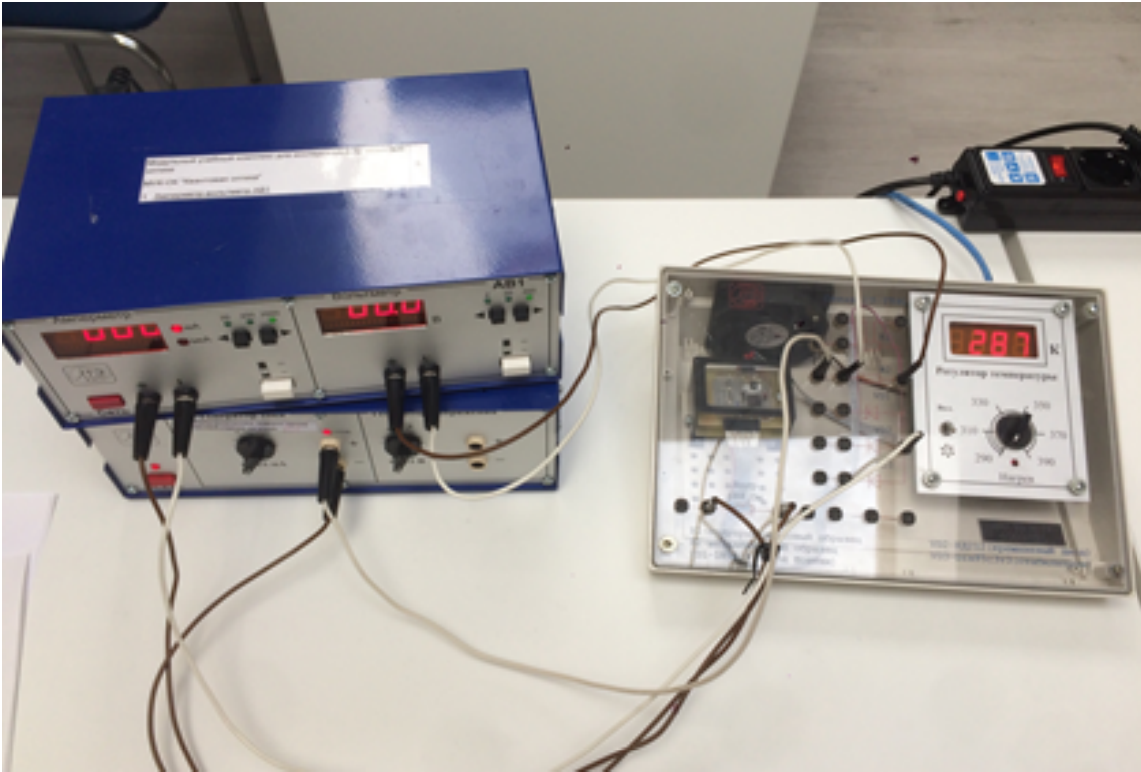
\includegraphics[width=0.9\linewidth]{img/3.5device.png}}
\end{minipage}
\begin{minipage}[h]{0.5\linewidth}
\center{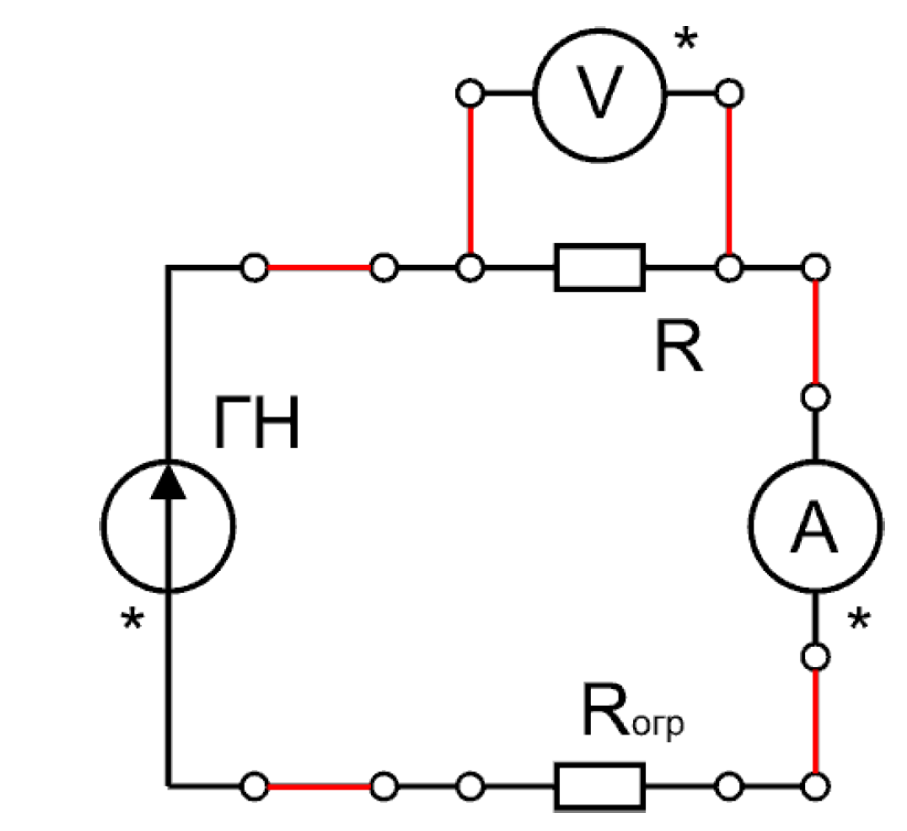
\includegraphics[width=0.8\linewidth]{img/3.5scheme.png}}
\end{minipage}
\caption{Общий вид установки и её принципиальная схема}
\end{figure}